\section{\cmtfinal{Panel Experiments with Staggered Rollouts} and Assumptions}\label{sec:experiment-outcome-estimand}
    In this section, we first introduce \cmtfinal{panel experiments with staggered rollouts} and then describe the two types of experiments that are considered in this paper. We also specify assumptions on the outcome model and treatment designs. Throughout, $[M]$ refers to the set $\{1, 2, \ldots, M\}$, for any positive integer $M$, {and additional notations used in the paper are summarized in Table \ref{tab:notations}}.
    

    Recall Examples \ref{ex:driver-safety}-\ref{ex:infectious-disease}, and assume
    we are planning to run an experiment to estimate the effect of a treatment of interest (app feature or public health intervention). 
    Let $z_{it}$ in $\{-1,+1\}$ be the treatment variable for unit $i$ at time $t$, for $i, t \in \mathbb{Z}$, where $z_{it} = +1$ means unit $i$ is treated at time $t$ and $z_{it} = -1$ means otherwise. Assume the treatment is not applied to any unit before the experiment starts, that is, $z_{it} \equiv -1$ for all $i$ and $t \leq 0$. The experimental designer decides the treatment assignments in an experiment with $N$ units over $T$ time periods, that is, chooses $z_{it}$ for $i \in [N]$ and $t \in [T]$. All the decision variables can be written in a compact form $Z = [z_{it}]_{(i,t)\in [N] \times [T]}$, which is referred to as the treatment design of the experiment. Different treatment designs lead to different panels of observed outcomes, denoted as $Y = [Y_{it}]_{(i,t)\in [N] \times [T]}$, that affect the precision of treatment effect estimates. The estimation precision, to be defined formally in Section \ref{subsec:objective}, directly impacts the cost of running the experiment since it specifies the required number of units and time periods. Therefore, optimizing the treatment decisions is an integral part of designing \cmtfinal{panel experiments}.
    
    In this paper, we consider two types of \cmtfinal{panel experiments}: non-adaptive experiments and adaptive experiments. For nonadaptive experiments, $N$ and $T$ are fixed, whereas for adaptive experiments, $N$ is fixed, but $T$ is unknown. Non-adaptive experiments enjoy the benefit of simplicity and involve the straightforward construction of statistical tests for the treatment effects. However, non-adaptive experiments can be inefficient in time and cost, as the experiment may run longer than needed to attain a certain precision of treatment effect estimates. In comparison, adaptive experiments can early stop the experiment if needed, at the expense of making statistical inference for treatment effects more challenging. We study the design of non-adaptive experiments in Section \ref{sec:model}, where treatment decisions are made before the experiment starts. Building on our insights from the non-adaptive experiments, we propose an algorithm in Section \ref{sec:sequential-experiment} to run adaptive experiments that make treatment decisions adaptively during the experiment and provide valid post-experiment inference of treatment effects.
    
    
\cmtfinal{We focus on a class of panel experiments whose treatment assignments satisfy the irreversible treatment adoption condition. These experiments with treatment adoption times possibly varying across units are referred to as panel experiments with staggered rollouts; the design of these experiments is referred to as the staggered rollout design.}
%
\begin{assumption}[Irreversible Treatment Adoption]\label{ass:treatment-adoption}
	For all $(i,t)\in [N]\times[T]$,
	$z_{it} \leq z_{i,t+1}$.
\end{assumption}
%
We mostly focus on the irreversible scenario for two reasons. First, often there are practical constraints
restricting units from switching between control and treatment, such as the policies or programs implemented at the group level ({\it e.g.}, city or state level), or the features that are electronically rolled to the user interface ({\it e.g.}, ride-hailing app feature). Second, when the treated units switch back to the control, they may not return to the original control status. For example, drivers may develop different driving habits via the new feature. In fact, the irreversible pattern is common in observational studies ({\it e.g.}, \cite{card1994minimum,abadie2010synthetic}).
In the experiment design literature, the irreversible pattern appears in the stepped wedge designs of cluster randomized trials in public health \citep{brown2006stepped,hussey2007design,woertman2013stepped,hemming2015stepped}, and in the synthetic control designs \citep{doudchenkodesigning2021,doudchenko2021synthetic,abadie2021synthetic}. 
%
\begin{remark}[Extension to Reversible Treatments]\label{rem:reversible}
In Section \ref{subsec:reversible-treatment}, we study the design of non-adaptive panel experiments when the treatment can be stopped. We show that optimizing the treatment designs for this case follows from our results in Section \ref{sec:model}.
\end{remark}


	\begin{figure}[t!]
	\begin{subfigure}{0.4\textwidth}
		\centering
		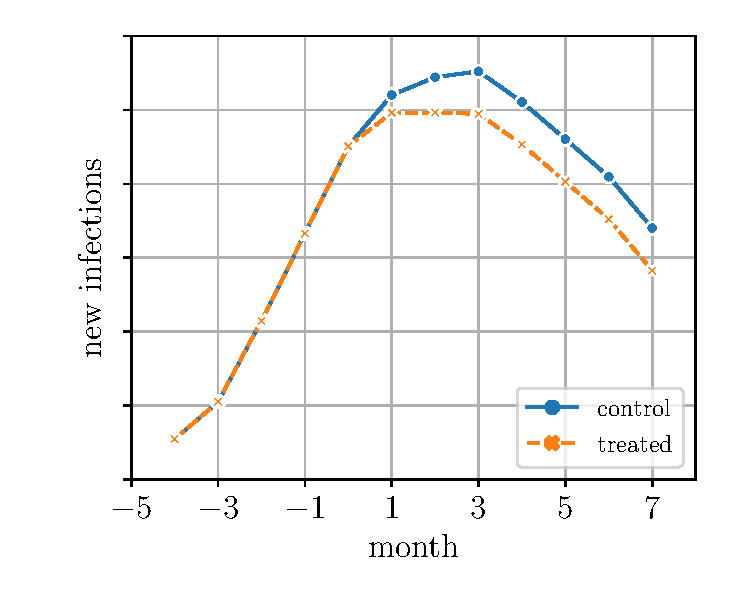
\includegraphics[width=1\linewidth]{plots/illustration/cumulative_effect_new_infection.pdf}
		\caption{Example 1}\label{fig:cumulative-effect} 
	\end{subfigure}\hfill
	\begin{subfigure}{0.4\textwidth}
		\centering
		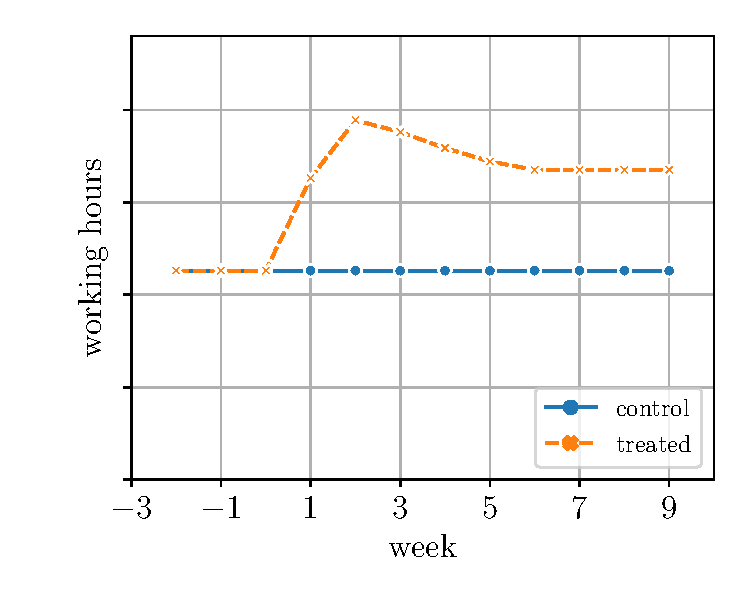
\includegraphics[width=1\linewidth]{plots/illustration/wearout_effect_app.pdf}
		\caption{Example 2}\label{fig:wearout-effect} 
	\end{subfigure}
	\vspace{2mm}
	\caption{\textbf{Illustrative examples of cumulative effects.} These figures show the cumulative effects $\tau_0 + \cdots + \tau_j$ as a function of the number of treated periods $j$. Figure \ref{fig:cumulative-effect} illustrates a scenario where the effect of a new public health intervention on new infections accumulates over time ($\tau_0, \tau_1, \tau_2 < 0$). Figure \ref{fig:wearout-effect} illustrates a scenario where the effect of a new app feature on drivers' working hours attenuates over time ($\tau_0, \tau_1 > 0$ and $\tau_2, \tau_3, \tau_4, \tau_5 < 0$). 
	}
	\label{fig:example}
\end{figure}



Next we introduce the potential outcome model. 

\begin{assumption}[Potential Outcome Model]\label{ass:model}
The potential outcomes for unit $i$ at time $t$ can be written as
\cmtrx{\[Y_{it}(z_{i,t-\ell}, \cdots, z_{i,t-1}, z_{it}) \]
for a nonnegative integer $\ell$, where $\ell$ is known.
}

\end{assumption}


Assumption \ref{ass:model} requires that a unit's treatment $z_{it}$ only affects this unit's own outcomes (no cross-unit interference). It further requires that a unit's outcomes are not affected by this unit's future treatment assignments (no anticipation). For example, drivers do not increase their working hours in anticipation of the new app feature. No anticipation is also commonly imposed in the literature \citep{basse2019minimax,bojinov2020design}. 

We allow the potential outcomes to depend on the treatment assignments up to $\ell$ periods in the past. \cmtrx{We assume $\ell$ is known for the design and estimation purposes. Note that there exists a bias-variance tradeoff in the specification of $\ell$ in practice. When the specified $\ell$ is less than the true value, the estimator can be biased. When the specified $\ell$ is more than the true value, the estimator is unbiased, but can be inefficient. See Figure \ref{fig:varying-ell} in Section \ref{ecsec:spec-ell} for an example. }


We define the average instantaneous effect $\tau_0$ and lagged effects $\tau_1,\dots,\tau_\ell$ as 
 \cmtrx{   \[ 
        \tau_j \coloneqq \frac{1}{NT} \sum_{i,t}   \frac{1}{2} \Big[ Y_{it}(-1, \cdots, -1, \underbrace{+1}_{z_{i,t-j}}, +1, \cdots, +1) - Y_{it}(-1, \cdots, -1, \underbrace{-1}_{z_{i,t-j}}, +1, \cdots, +1) \Big]\,,
 \]}
 for all $j\in \{0\} \cup [\ell]$. 
 Here $1/2$ is used for notation simplicity in the specification \eqref{eqn:model-setup} below and remaining sections to account for the scaling of $z_{it}$ that takes value between $\{+1,-1\}$ as opposed to $\{+1,0\}$. Note that $\tau_j$ is the average, over individuals and time periods, of individual-time specific treatment effects that can be heterogeneous in both units and time periods.


Here $\tau_0, \tau_1, \cdots, \tau_\ell$ can take arbitrary values, and therefore allow for general dynamics of cumulative effects over time. To demonstrate this generality, we describe a few scenarios below.
	%
	\begin{itemize}
	    \item The average effect accumulates over time, for example when $\tau_0,\ldots,\tau_\ell$ all have the same sign, as shown in Figure \ref{fig:cumulative-effect}.
	    
	    \item The average effect attenuates over time, for example when $\tau_0$ and $\tau_1$ have a different sign than all of $\tau_2,\ldots,\tau_\ell$, as shown in Figure \ref{fig:wearout-effect}.
	    
	    \item The average effect is constant over time, for example when $\ell = 0$.
	    
	    \item The average cumulative effect is zero, for example when $\sum_{j=0}^\ell \tau_j=0$. After $\ell$ periods, a unit's outcome is the same as the outcome of never being treated. 
	    
	\end{itemize}
	
		In this paper, we are interested in estimating $\bm{\tau} = (\tau_0, \tau_1, \cdots, \tau_\ell)$. Below we study how to choose $Z = [z_{it}]_{(i,t)\in [N]\times[T]}$
		to accurately estimate these parameters.